\chapter{GMS}
\label{ch:one}

\section{Case Study: the GMS model}

The Gierer-Meinhardt system \cite{gierer_theory_1972}, with saturation, is given by the following pair of nonlinear pdes; a system in a family sometimes referred to as reaction-diffusion equations:
% 
\begin{equation}
\label{eqn:o-gms1}
\begin{split}
\begin{aligned}
	u_t &= D_u\De u + a(u,v) = D_u\De u - u +\frac{u^2}{v(1+ku^2)} \\
	\tau v_t &= D_v\De v + b(u,v) = D_v\De v - v + u^2,
\end{aligned}
\end{split}
\end{equation}
% 
with $D_u = \Ep^2, D_v = D/\Ep$, plus homogeneous Neumann boundary conditions on $x\in[0,1]$. We consider the limit where $\Ep\ll 1$, and regard all the other constants as being $O(1)$. 

\subsection{Construction of the solution in the near-shadow limit}

For the near-shadow limit, $D=\DD/\Ep$, we want to construct a $K-$stripe stationary solution on $x\in[0,1]$, with $L=1/K$ the period of the solution, and $l$ the length of each individual mesa, as shown in figure \eqref{fig:single_mesa}.
% 
\begin{figure}[htb]
\begin{center}
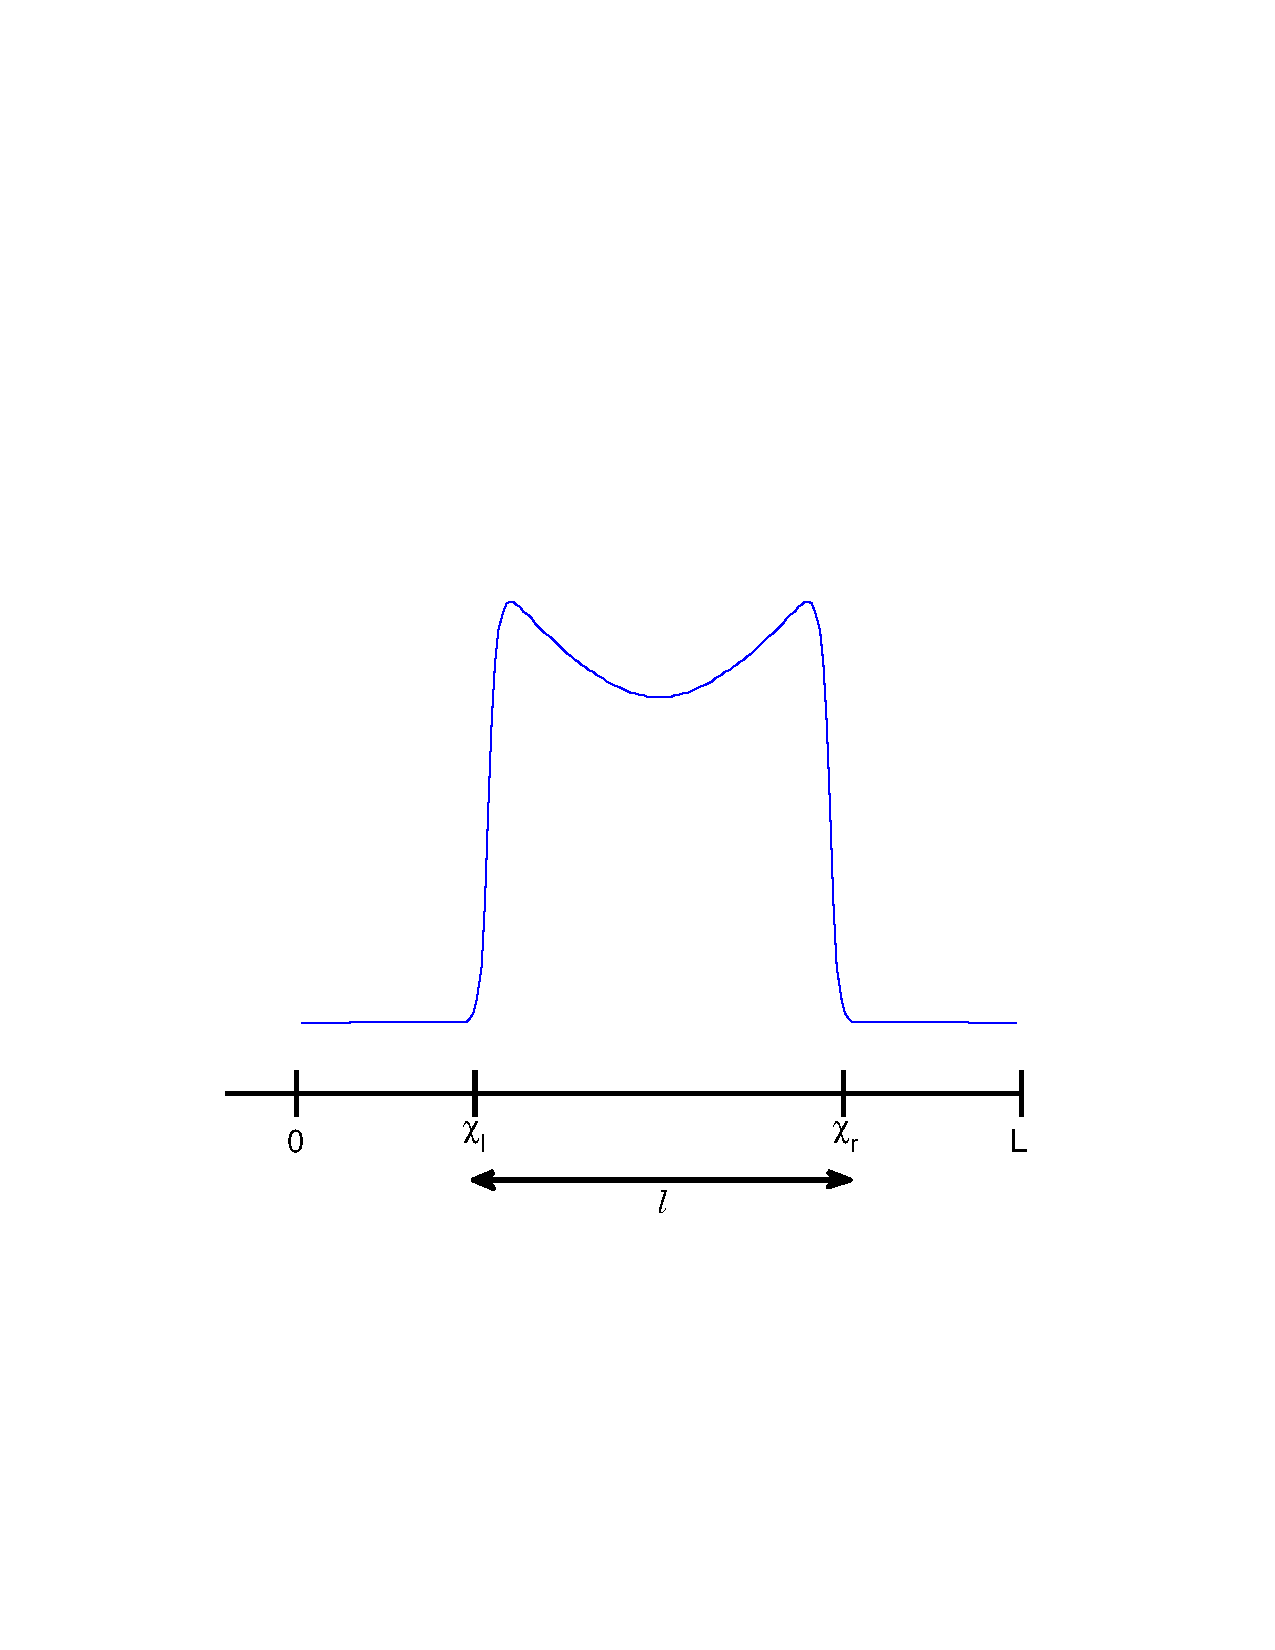
\includegraphics[width=4in]{single_mesa}
\caption{A typical mesa profile in the stationary solution $v(x)$. The left and right edges of the mesa are labelled as $\chi_l$ and $\chi_r$ respectively; and the length of the mesa section is $l$.}
\label{fig:single_mesa}
\end{center}
\end{figure}
% 
The stationary equation we want to solve is
% 
\begin{equation}
\label{eqn:o-gms_stat}
\begin{split}
\begin{aligned}
	0 &= \Ep^2 u_{xx} -u + \frac{u^2}{v(1+ku^2)},\qquad &u_x(0)=u_x(L)=0, \\
	0 &= \frac{\DD}{\Ep}v_{xx} - v + u^2,\qquad &v_x(0)=v_x(L)=0.
\end{aligned}
\end{split}
\end{equation}
% 

***did not define $g(u,v)=\frac{u^2}{v(1+ku^2)}$, as it's only used much further down the road***

To first order, we have in the $v$ equation that $v_{xx}=0$. Applying the Neumann condition, we have then that $v\sim\VV$, and the value of the constant can be estimated by integrating over the whole domain,
% 
\begin{equation}
\label{eqn:o-v_first_order}
  \VV = \frac{1}{L}\int_0^Lu^2dx.
\end{equation}
% 

In the inner region near the left boundary of the mesa we have that $v=\VV$, and we do a change of variables for $u=\VV w$ and $y=\Ep^{-1}(x-\chi_l)$. The resulting equation is
% 
\begin{equation}
\label{eqn:o-w_eqn}
  w_{yy}+f(w)=0, \qquad -\infty<y<\infty,\qquad f(w) = -w + \frac{w^2}{1+bw^2},
\end{equation}
% 
with $b = k\VV^2$. Now, we are looking for a heteroclinic connection in $u$ as the transition mechanism that generates the mesa, one for the each side of the mesa. For a heteroclinic connection to exist in \eqref{eqn:o-w_eqn}, it has to satisfy the Maxwell line condition \cite{maxwell1994}.
% 
\begin{figure}[htb]
\begin{center}
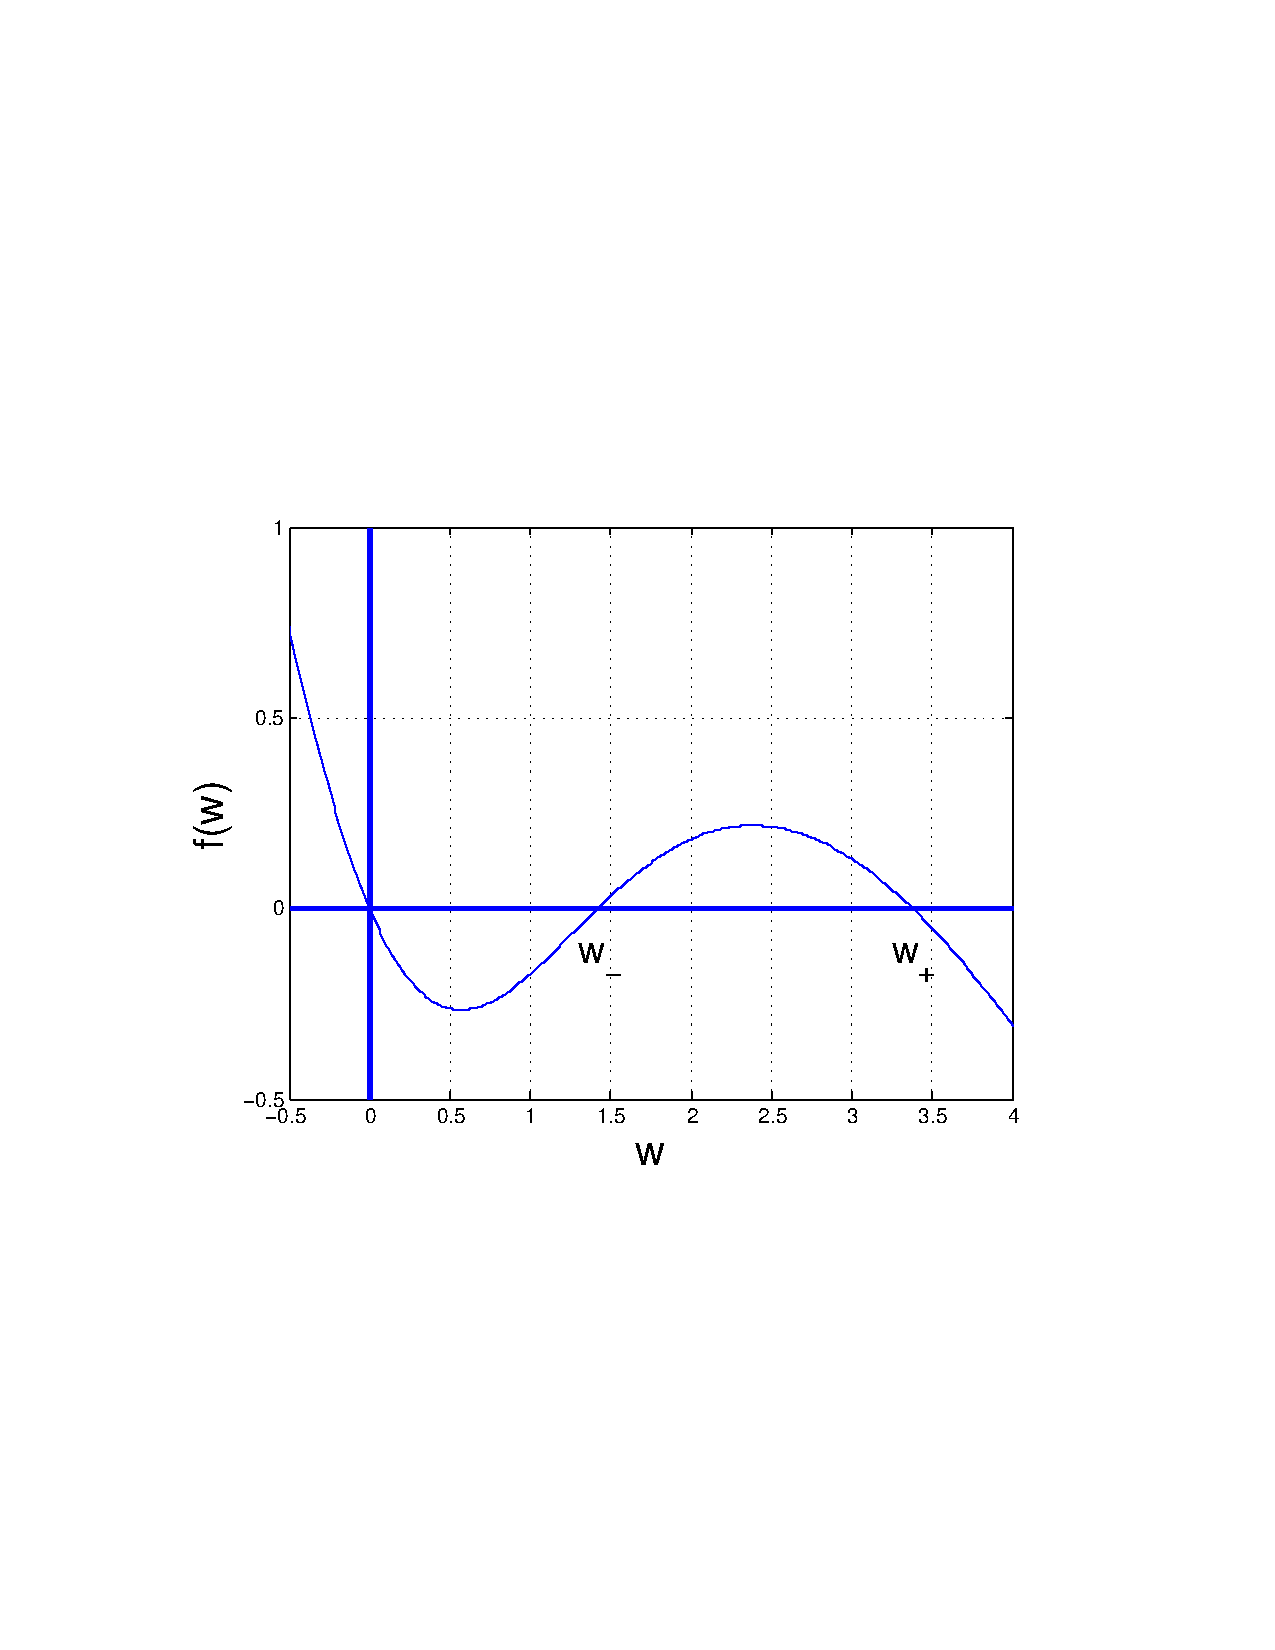
\includegraphics[width=4in]{f_of_w}
\caption{A plot of the function $f(w)$ given in \eqref{eqn:o-w_eqn}.}
\label{fig:f(w)}
\end{center}
\end{figure}
% 

The function $f(w)=0$ has zeros at $w=0$ and $w_{\pm} = \frac{1\pm\sqrt{1-4b}}{2}$, with distinct real values for $w_{\pm}$ existing in the range $0\le b<1/4$. The profile of the curve in that range can be seen in figure \eqref{fig:f(w)}. The Maxwell line condition states that a heteroclinic connection will exist for the value $b=b_0$ such that $\int_0^{w_+} f(w)dw = 0$. Integrating $f(w)$ we get
% 
\begin{equation*}
% \label{eqn:maxwell_lc}
\begin{split}
\begin{aligned}
  \int_0^{w_+} f(w)dw &= \left.\left(-\frac{w^2}{2} + \frac{w}{b} - \frac{1}{b^{3/2}}\arctan(b^{1/2}w) \right)\right|_0^{w_+},\\
  & = -\frac{w_+^2}{2} + \frac{w_+}{b_0} - \frac{1}{b_0^{3/2}}\arctan(b_0^{1/2}w_+),
\end{aligned}
\end{split}
\end{equation*}
% 
and since we have that $b_0 = \frac{w_+-1}{w_+^2}$, the Maxwell line condition will be satisfied if
% 
\begin{equation}
\label{eqn:maxwell2}
b_0 = \frac{w_+-1}{w_+^2},\qquad \sqrt{w_+-1}(w_++1)=2w_+\arctan(\sqrt{w_+-1}).
\end{equation}

This can be solved numerically to obtain the critical values $b_0 = 0.211376$, and $w_+ = 3.295209$. (??? do a plot of numerical vs asymptotic approximation)

For use later in section \eqref{section:stability}, we need to compute
% 
$$
\beta = \int_{-\infty}^{\infty}w'^2dy
$$
% 

We multiply \eqref{eqn:o-w_eqn} by $w'$ to get 
% 
\begin{equation*}
  \frac{d}{dy}\left(\frac{w'^2}{2} \right)=\frac{d}{dy}\mathcal{F}(w)\qquad\rightarrow\qquad w'^2 = 2\mathcal{F},
\end{equation*}
% 
with $\mathcal{F} = \int_0^wf(s)ds$. We then get
% 
\begin{equation}
\label{eqn:o-beta}
  \beta = \int_{-\infty}^{\infty}w'^2dy = \int_{0}^{w_+}w'^2\frac{1}{w'} dw = \int_{0}^{w_+}\sqrt{2\mathcal{F}(w)}dw.
\end{equation}
% 

This can be numerically calculated using the previously computed value for $w_+$, to get $\beta\sim1.49882$.

Linearizing around $w=0$ for $y\rightarrow -\infty$, and for $w=w_+$ for $y\rightarrow \infty$, we get that for $b=b_0$ we have a heteroclinic solution 
% 
\begin{equation*}
% \label{eqn:hetero}
\begin{split}
\begin{aligned}
  &w''+f(w)=0,\qquad &-\infty<y&<\infty,\qquad f(w) = -w + \frac{w^2}{1+b_0w^2},\\
  &w\sim d_-e^y,\qquad &&\mathrm{as}\hspace{2pt}y\rightarrow -\infty,\\
  &w\sim w_+ - d_+e^{-\nu_+y},\qquad&&\mathrm{as}\hspace{2pt}y\rightarrow \infty,
\end{aligned}
\end{split}
\end{equation*}
% 
for $\nu_+ = \sqrt{1-2/w_+}$. By translation we take $w(0)=w_+/2$, in order to have uniqueness.

A full mesa solution will consist of two back-to-back heteroclinic curves, and can be constructed as
% 
\begin{equation*}
  u\sim \VV[w_l + w_r - w_+],\qquad  \textrm{with }w_l\sim w\left(\frac{x-\chi_l}{\Ep}\right),\qquad w_r\sim w\left(\frac{\chi_r-x}{\Ep}\right).
\end{equation*}
% 

Integrating \eqref{eqn:o-v_first_order}, we get that to first order $\VV\sim\frac{1}{L}\VV^2w_+^2l$, with $l=\chi_r-\chi_r$ the width of the mesa. We then have
% 
\begin{equation*}
  \VV w_+^2\sim\frac{L}{l} + O(\Ep),\qquad l\sim\frac{L\sqrt{k}}{\sqrt{b_0}w_+^2}<L,
\end{equation*}
% 
therefore a necessary condition for a $K-$stripe solution to exist is that 
% 
\begin{equation*}
  \frac{\sqrt{k}}{\sqrt{b_0}w_+^2}<1.
\end{equation*}
% 

To refine the solution, it is necessary to further expand $u(x)$ and $v(x)$. In the outer region we expand $u$ and $v$ as
$$
v\sim \VV + \Ep v_1 + \Ep^2 h_2 + \cdots.
$$

Since outside of the mesa $u$ is exponentially small, and in the plateau region $u\sim\VV w_+ + O(\Ep)$, by substituting into \eqref{eqn:o-gms_stat}, we get that
% 
\begin{equation}
\label{eqn:o-v1}
	\begin{split}
	\DD v_{1,xx}
   = \left\{
	\begin{matrix}
		\VV& \mathrm{for}\hspace{2pt}0< x<\chi_l \\
		\VV(1-\VV w_+^2) = \VV(1-L/l)& \mathrm{for}\hspace{2pt}\chi_l< x<\chi_r\\
		\VV& \mathrm{for}\hspace{2pt}\chi_r<x<L
	\end{matrix}\right.
	\end{split}
\end{equation}
% 
with $v_{1,x}(0) = v_{1,x}(L) = 0$. In order to find the conditions on $v_1$ at the transition layers $\chi_l$ and $\chi_r$, we expand $u$ as $u\sim\VV w_+ + \Ep\UU_1 + ...$ on $\chi_l<x<\chi_r$.

Substituting into \eqref{eqn:o-gms_stat}, we get that 
\[
-\UU_1 + g_u(\VV w_+,\VV)\UU_1 + g_v(\VV w_+,\VV)v_1 = 0.
\]

Since $1+b_0w_+^2 = w_+$, the linearization terms simplify to
% 
\begin{equation}
\label{eqn:derivs}
\begin{split}
\begin{aligned}
  g_u(\VV w_+,\VV) = \frac{2w_+}{(1+b_0w_+^2)^2} = \frac{2}{w_+},\\
  g_v(\VV w_+,\VV) = \frac{-w_+^2}{1+b_0w_+^2} = -w_+,
\end{aligned}
\end{split}
\end{equation}
% 
and this yields
$$
-\UU_1 + \frac{2}{w_+}\UU_1 - w_+v_1 = 0,\qquad \Rightarrow \qquad \UU_1 = \frac{w_+^2}{2-w_+}v_1.
$$

We now expand $u$ and $v$ near the $x=\chi_l$ $(y=\Ep^{-1}(x-\chi_l))$ as
% 
\begin{equation*}
  u = u_0 + \Ep u_1 + \Ep^2 u_2+ \cdots,\qquad v = \VV + \Ep\VV_1 + \Ep^2\VV_2+\cdots,
\end{equation*}
% 
with $u_0 = \VV w_+$. Substituting into \eqref{eqn:o-gms_stat}, the $O(\Ep)$ system is
% 
\begin{equation}
\label{eqn:ord_epsilon}
\begin{split}
\begin{aligned}
  \LL u_1:&\equiv u_1''-u_1 + g_u(u_0,\VV)u_1 = -g_v(u_0,\VV)\VV_1 \\
  \VV_1'' &= 0.
\end{aligned}
\end{split}
\end{equation}
% 

For $\VV_1$ we get that $\VV_1 = \VV_{10} + \VV_{11}y$. We have that $\LL a_0' = 0$.

The solvability condition on \eqref{eqn:ord_epsilon} is then that 
% 
\begin{equation}
\label{eqn:solvab}
\begin{split}
\begin{aligned}
\int_{-\infty}^{\infty}g_v(u_0,\VV)\VV_1u_0'dy = \int_{-\infty}^{\infty}\frac{w^2}{1+bw^2}w'\VV_1dy = 0.
\end{aligned}
\end{split}
\end{equation}
% 

Substituting in $\VV_1 = \VV_{10} + \VV_{11}y$, the condition from \eqref{eqn:solvab} implies that
% 
\begin{equation*}
% \label{eqn:solvab2}
\begin{split}
\begin{aligned}
\VV_{10}\int_{-\infty}^{\infty}\frac{w^2w'}{1+bw^2}dy + \VV_{11}\int_{-\infty}^{\infty}\frac{w^2w'y}{1+bw^2}dy = 0.
\end{aligned}
\end{split}
\end{equation*}
% 

Since $\VV_1 = O(\Ep)$, $\VV_{11}$ has to be zero, as otherwise for $|y|\gg 1$ we would have $\VV_1 = O(1)$. Consequently, $\VV_{10}$ also has to be zero, and the conclusion is that $\VV_1=0$. We have then that $\LL u_1 = 0$, and therefore we also have $u_1 = 0$

This result yields that 
% 
\begin{equation*}
  v_1(\chi_l)  = v_1(\chi_r) = 0,
\end{equation*}
% 
and now we have enough conditions to solve uniquely for $v_1$.

Using the fact that $\chi_r-\chi_l = l$, and that $\VV w_+^2 = L/l$, the full solution to \eqref{eqn:o-v1} is
% 
\begin{equation*}
% \label{eqn:v1_full}
	\begin{split}
	v_1
   = \left\{
	\begin{matrix}
		\frac{\VV}{2\DD}(x^2-\chi_l^2)& \mathrm{for}\hspace{2pt}0< x<\chi_l \\
		\frac{\VV(l-L)}{2\DD l}[(x-\chi_l)^2 - l(x-\chi_l)]& \mathrm{for}\hspace{2pt}\chi_l< x<\chi_r\\
		\frac{\VV}{2\DD}[(L-x)^2-(L-\chi_r)^2]& \mathrm{for}\hspace{2pt}\chi_r<x<L
	\end{matrix}\right.
	\end{split}
\end{equation*}
% 

It is possible now to calculate $v_{1,x}$ close to the transition layers. We have
% 
\begin{equation}
\label{eqn:v1x}
\begin{split}
\begin{aligned}
  v_{1,x}(\chi_l^-) = \frac{\VV\chi_l}{\DD},\qquad &v_{1,x}(\chi_l^+) = \frac{\VV(L-l)}{2\DD},\\
  v_{1,x}(\chi_r^-) = -\frac{\VV(L-l)}{2\DD},\qquad &v_{1,x}(\chi_r^+) = -\frac{\VV(L-\chi_r)}{\DD},\\
\end{aligned}
\end{split}
\end{equation}
% 

% From equilibrium theory (ref ???), we have that $v_{1,x}(\chi_l^-) = v_{1,x}(\chi_l^+)$, as well as $v_{1,x}(\chi_r^-) = v_{1,x}(\chi_r^+)$. This yields that $\chi_l = \frac{L-l}{2}$, and $\chi_r = \frac{L+l}{2}$.

This suggests that there is a term to next order, as $\VV_2\sim v_{1,x}(\chi_l)$. Expanding to next order in the inner region, as $u = u_0 + \Ep^2u_2$ and $v = \VV + \Ep^2\VV_2$, and defining $g_0(w) = \frac{w^2}{1+b_0w^2}$, we have the system
% 
\begin{equation*}
% \label{eqn:solva2}
\begin{split}
\begin{aligned}
  \LL u_2 =  u_2'' - u_2 + g_0'(w)u_2 = g_0(w)\VV_2,\\
  \VV_2'' = 0.
\end{aligned}
\end{split}
\end{equation*}
% 

We have then that $\VV_2 = \VV_{20} + y\VV_{21}$. 

We can derive a solvability condition from $\LL u_2 = g_0(w)\VV_2$, since $\LL w'=0$. We get
% 
\begin{equation*}
  \int_{-\infty}^{\infty}\VV_2g_0(w)w'dy = \int_{-\infty}^{\infty}(\VV_{20} + y\VV_{21})g_0(w)w'dy = 0,
\end{equation*}
% 

We can now match the inner solution to the outer solution evaluated at the interface, to determine $\VV_{20}$ and $\VV_{21}$. We get that
% 
\begin{equation*}
  \VV + \Ep^2(\VV_{20} + y\VV_{21}) + \cdots = \VV + \Ep v_1(\chi_l) + \Ep v_{1,x}(\chi_l^-)(x-\chi_l) + \Ep^2v_2(\chi_l)+\cdots
\end{equation*}
% 

From this we can conclude that $\VV_{21} = v_{1,x}(\chi_l^-)$, and that $\VV_{20} = v_2(\chi_l)$. This last value, for both the inner and outer solutions, can be calculated from the solvability condition given that we now know $\VV_{21}$. 

Furthermore, repeating the matching procedure with $x\rightarrow \chi_l^+$ yields the same value, as the outer solution has no ambiguity. From this we get that $v_{1,x}(\chi_l^+) = v_{1,x}(\chi_l^-)$. Repeating the procedure yet again at the right boundary $\chi_r$, we get the same result, i.e., $v_{1,x}(\chi_r^+) = v_{1,x}(\chi_r^-)$. Since we already knew from \eqref{eqn:v1x} that $v_{1,x}(\chi_l^+) = - v_{1,x}(\chi_r^-)$, we can solve for $\chi_l$ and $\chi_r$ to get that the position of the boundaries of the mesa on $[0,L]$ are
% 
$$
  \chi_l = \frac{L-l}{2}, \qquad \chi_r = \frac{L+l}{2},
$$
% 
with $l$ the length of the plateau. A corollary from this result is that that stationary mesa solutions have to be centred.

We can find a second solvability condition that will be of use later on. Differentiating with respect to $y$, we have
% 
\begin{equation*}
  \LL u_2' = -g_0''(w)u_2w' + g_0(w)\VV_2' + g_0'(w)\VV_2w',
\end{equation*}
% 
and using the fact that $\LL w'=0$, the solvability condition we get is
% 
\begin{equation}
\label{eqn:solva1}
\begin{split}
\begin{aligned}
  -\VV_{21}\int_{-\infty}^{\infty}g_0(w)w'dy = \int_{-\infty}^{\infty}(g_0'(w)\VV_2 - g_0''(w)u_2)w'^2dy,\\
  v_{1,x}(\chi_r)\int_{-\infty}^{\infty}g_0(w)w'dy = \int_{-\infty}^{\infty}(g_0'(w)\VV_2 - g_0''(w)u_2)w'^2dy,
\end{aligned}
\end{split}
\end{equation}
% 
since $\VV_2' = \VV_{21} = -v_{1,x}(\chi_r)$.


\subsection{\label{section:stability}Stability in the near-shadow limit to perturbations in the y direction}

We assume that the solutions exist in a rectangular domain $[0,1]\times[0,d_0]$, with Neumann boundary conditions on all sides. We introduce a perturbation on the equilibrium solution $(u_e,v_e)$ of the form
% 
\begin{equation*}
  u = u_e + e^{\lA timy}\phi(x),\qquad v = v_e + e^{\lA timy}\psi(x); \qquad m = \frac{k\pi}{d_0},k=1,2,\ldots,
\end{equation*}
%
with $|\phi(x)|\ll1$, and $|\psi(x)|\ll1$.

Substituting into \eqref{eqn:o-gms1}, we get the following eigenvalue problem
%
\begin{subequations}
\begin{align}
\label{eqn:eigen_gms1}
  \bar{\lA}\phi = \LL_{\Ep}\phi + g_v(u_e,v_e)\psi &= \Ep^2\phi_{xx} - \phi + g_u(u_e,v_e)\phi + g_v(u_e,v_e)\psi,\\
\label{eqn:eigen_gms2}
  \frac{\Ep}{\DD}(1+\tau\lA)\psi &= \psi_{xx} - m^2\psi + \frac{2\Ep}{\DD}u_e\phi,
\end{align}
\end{subequations}
% 
with $\bar{\lA} = \lA + \Ep^2m^2$, and Neumann conditions $\phi_x(0)=\phi_x(1)=\psi_x(0)=\psi_x(1)=0$.

As shown in \eqref{eqn:derivs}, in the plateau region we have that $g_u(u_e,v_e) = 2/w_+$, and $g_v(u_e,v_e) = -w_+$. Substituting into \eqref{eqn:eigen_gms1}, we have that, to first order, when $\bar{\lA}\ll 1$ (???), the asymptotic form of $\phi$ on the plateau region is 
% 
\begin{equation*}
  \phi = \mu\psi,\qquad \textrm{with  }\mu \equiv \frac{w_+^2}{2-w_+},\qquad \chi_l<x<\chi_r.
\end{equation*}
% 
Outside of the plateau region $\phi$ is asymptotically small, therefore near the transition layers located at $\chi_l,\chi_r$, $\phi$ is proportional to the derivative $w'$ of the heteroclinic connection. We have then the following asymptotic form for $\phi$
% 
\begin{equation*}
% \label{eqn:phi_asy2}
	\begin{split}
	\phi
   \sim \left\{
	\begin{matrix}
		c_{li}(w'(\Ep^{-1}(x-\chi_{li}))+O(\Ep))& \mathrm{for}\hspace{2pt} x\sim\chi_{li}& \\
		c_{ri}(w'(\Ep^{-1}(\chi_{ri}-x))+O(\Ep))& \mathrm{for}\hspace{2pt} x\sim\chi_{ri}& \\
		\phi_i = \mu\psi& \mathrm{for}\hspace{2pt}x\in(\chi_{li},\chi_{ri}),&i=1,\hdots,K,
	\end{matrix}\right.
	\end{split}
\end{equation*}
% 
with the constants $c_{li},c_{ri}$ to be found.

Since $\phi$ is localized near the transition layers, we can estimate it in the sense of distributions, approximating $u_e$ as $u_e\sim\VV w$
% 
\begin{equation*}
\begin{split}
\begin{aligned}
  \frac{2\Ep u_e\phi}{\DD}&\sim \frac{2\Ep^2\VV c_l}{\DD}\int_{-\infty}^{\infty}w_lw_l'dy\dE(x-x_l) +...\\ 
  &\qquad+\frac{2\Ep^2\VV c_r}{\DD}\int_{-\infty}^{\infty}w_rw_r'dy\dE(x-x_r) + \frac{2\Ep\VV}{\DD}w_+\mu\psi H_{[\chi_l,\chi_r]},
\end{aligned}
\end{split}
\end{equation*}
% 
with $H_{[\chi_l,\chi_r]} = 1$ on $x\in (\chi_l,\chi_r)$, and zero elsewhere.

This then yields
% 
\begin{equation*}
% \label{eqn:phi_main}
\begin{split}
\begin{aligned}
\frac{2\Ep u_e\phi}{\DD}&\sim \frac{\Ep^2\VV c_lw_+^2}{\DD}\dE(x-x_l) +\frac{\Ep^2\VV c_rw_+^2}{\DD}\dE(x-x_r) + \frac{2\Ep\VV w_+\mu\psi H}{\DD}
\end{aligned}
\end{split}
\end{equation*}
% 
Substituting into \eqref{eqn:eigen_gms2}, we get that $\psi$ satisfies
% 
\begin{equation}
\label{eqn:phi_main2}
\begin{split}
\begin{aligned}
\psi_{xx}-\tH^2\psi = -\frac{\Ep^2\VV w_+^2}{\DD}\left[\sum_i(c_{li}\dE(x-\chi_{li}) + c_{ri}\dE(x-\chi_{ri})) \right],
\end{aligned}
\end{split}
\end{equation}
% 
with $\tH$ the piecewise constant function
% 
\begin{equation}
\label{eqn:phi_asym}
	\begin{split}
	\tH
   = \left\{
	\begin{matrix}
		\tH_-\equiv\left(m^2+\frac{\Ep(1+\tau\lA)}{\DD}\right)^{1/2},& \mathrm{for}\hspace{2pt} x\notin\cup_{i=1}^K[\chi_{li},\chi_{ri}]\\
		\tH_+\equiv\left(m^2+\frac{\Ep(1+\tau\lA)}{\DD}\left(1+\frac{2w_+}{l(w_+-2)} \right)\right)^{1/2},& \mathrm{for}\hspace{2pt} x\in\cup_{i=1}^K[\chi_{li},\chi_{ri}]
	\end{matrix}\right.
	\end{split}
\end{equation}
% 

Since $w'$ is localized, we can define $w'_{li}=w'(x-\chi_{li})$ and $w'_{ri}=w'(\chi_{ri}-x)$, and multiply it into \eqref{eqn:eigen_gms1}, to obtain the matrix eigenvalue problem
% 
\begin{equation}
\label{eqn:matrix_eigen_l}
  c_{li}(w'_{li},\LL_{\Ep}w'_{li}) + (w'_{li},g_v(u_e,v_e)\psi) = c_{li}\bar{\lA}(w'_{li},w'_{li}),
\end{equation}
% 
and similarly
% 
\begin{equation}
\label{eqn:matrix_eigen_r}
  c_{ri}(w'_{ri},\LL_{\Ep}w'_{ri}) + (w'_{ri},g_v(u_e,v_e)\psi) = c_{ri}\bar{\lA}(w'_{ri},w'_{ri}),
\end{equation}
% 
where $(f,g) = \int_0^1fgdx$.

The second term in \eqref{eqn:matrix_eigen_l} and \eqref{eqn:matrix_eigen_r} can be readily estimated, using the fact that $w''-w = g_0(w)$, and that $g_v=-g_0$, as
% 
\begin{equation*}
\begin{split}
\begin{aligned}
% \label{eqn:2ndterml}
  (w'_{li},g_v(u_e,v_e)\psi) = \int_0^1 w_{li}'\psi g_v(u_e,v_e)dx  =-\Ep\psi(\chi_l)\int_{-\infty}^{\infty}w'g_0(w)dy  \\
  =-\Ep\psi(\chi_l)\int_{-\infty}^{\infty}w'(w''-w)dy = -\Ep\psi(\chi_l)\frac{w_+^2}{2},
\end{aligned}
\end{split}
\end{equation*}
% 
and similarly, 
% 
\begin{equation*}
\begin{split}
\begin{aligned}
% \label{eqn:2ndtermr}
  (w'_{ri},g_h(u_e,v_e)\psi) = -\Ep\psi(\chi_r)\frac{w_+^2}{2}.
\end{aligned}
\end{split}
\end{equation*}
% 

The third term can be estimated straight from the definition of $\beta$ in \eqref{eqn:o-beta}. We get
% 
\begin{equation*}
\begin{split}
\begin{aligned}
% \label{eqn:third term}
  (w'_{li},w'_{li})) \sim \Ep\int_{-\infty}^{\infty}(w')^2dy = \Ep\beta.
\end{aligned}
\end{split}
\end{equation*}
% 

The first term can be estimated using some of the results previously obtained. We have that 
% 
\begin{equation*}
  \LL_{\Ep}w_l'=(w_l')''-w_l'+g_u(u_e,v_e)w_l'.
\end{equation*}
%

We can approximate $g_u(u_e,v_e)$ as 
% 
\begin{equation*}
g_u(u_e,v_e)\sim g_u(w\VV,\VV) + \Ep^2(g_{uu}(w\VV,\VV) + g_{uv}(w\VV,\VV))+\cdots.
\end{equation*}
% 
The derivatives can be related to $g_0(w) = \frac{w^2}{1+b_0w^2}$ in the following way:
% 
\begin{equation*}
\begin{split}
\begin{aligned}
% \label{eqn:derivs_g}
  g_u(u,v)&=\frac{2u}{v(1+ku^2)^2}\sim\frac{2w}{(1+b_0w^2)^2}=g_0'(w),\\
  g_{uu}(u,v)&=\frac{1}{v}\frac{2-6ku^2}{(1+ku^2)^3}\sim\frac{1}{\VV}\frac{2-6b_0w^2}{(1+b_0w^2)^3}=\frac{1}{\VV}g_0''(w),\\
  g_{uv}(u,v)&=-\frac{2u}{v^2(1+ku^2)^2}\sim-\frac{2w}{\VV(1+b_0w^2)^2}=-\frac{1}{\VV}g_0'(w).
\end{aligned}
\end{split}
\end{equation*}
% 

Substituting them in, we get
% 
\begin{equation*}
\begin{split}
\begin{aligned}
  g_u(u_e,v_e)\sim g_0'(w)+\frac{\Ep^2}{\VV}(g_0''(w)u_2 - g_0'(w)\VV_2)+\cdots,\\
  \LL_{\Ep}w_{li}' \sim \frac{\Ep^2}{\VV}(g_0''(w_{li})u_2 - g_0'(w_{li})\VV_2)w_{li}'.
\end{aligned}
\end{split}
\end{equation*}
%

We then get for the first term
% 
\begin{equation*}
\begin{split}
\begin{aligned}
  (w'_{li},\LL_{\Ep}w'_{li}) &\sim \frac{\Ep^2}{\VV}\int_0^1\left(g_0''(w_{li})u_2 - g_0'(w_{li})\VV_2 \right)w_{li}'^2dx \\
  &\qquad= \frac{\Ep^3}{\VV}\int_{-\infty}^{\infty}\left(g_0''(w_{li})u_2 - g_0'(w_{li})\VV_2 \right)w_{li}'^2dy
\end{aligned}
\end{split}
\end{equation*}
% 

Using the solvability condition in \eqref{eqn:solva1}, 
% 
\begin{equation*}
\begin{split}
\begin{aligned}
  \VV_2'\int_{-\infty}^{\infty}g_0(w)w'dy = \int_{-\infty}^{\infty}(g_0'(w)\VV_2 - g_0''(w)u_2)w'^2dy,
\end{aligned}
\end{split}
\end{equation*}
% 
we get
% 
\begin{equation*}
\begin{split}
\begin{aligned}
  (w'_{li},\LL_{\Ep}w'_{li}) &\sim \frac{\Ep^3}{\VV}\VV_2'\int_{-\infty}^{\infty}g_0(w)w'dy = \frac{\Ep^3}{\VV}\VV_2'\int_{-\infty}^{\infty}(w-w'')w'dy\\
  &\qquad = \frac{\Ep^3\VV_2'}{2\VV}w_+^2 = \frac{\Ep^3v_{1x}(\chi_{li})w_+^2}{2\VV}
\end{aligned}
\end{split}
\end{equation*}
% 

Similarly, on the other side of the plateau the process is identical, except for a sign change in the slope,
% 
\begin{equation*}
\begin{split}
\begin{aligned}
  (w'_{ri},\LL_{\Ep}w'_{ri}) &\sim -\frac{\Ep^3v_{1x}(\chi_{ri})w_+^2}{2\VV}
\end{aligned}
\end{split}
\end{equation*}
% 

Putting everything together results in the following $2K\times 2K$ system
% 
\begin{equation*}
% \label{eqn:system0}
\begin{split}
\begin{aligned}
  \Ep\bar{\lA} c_{li}\beta &\sim \frac{\Ep^3}{2\VV}c_{li}v_{1x}(\chi_{li})w_+^2 - \frac{\Ep}{2}\psi(\chi_{li})w_+^2,\\
  \Ep\bar{\lA} c_{ri}\beta&\sim - \frac{\Ep^3}{2\VV}c_{ri}v_{1x}(\chi_{li})w_+^2 - \frac{\Ep}{2}\psi(\chi_{ri})w_+^2,
\end{aligned}
\end{split}
\end{equation*}
% 
and since from \eqref{eqn:v1x} we know that 
% 
\[
  v_{1x(\chi_{li})} = \frac{\VV(L-l)}{2\DD},
\]
% 
the above system can be simplified to 
% 
\begin{equation}
\label{eqn:system1}
\begin{split}
\begin{aligned}
  \bar{\lA}\beta c_{li} &\sim \Ep^2\frac{(L-l)w_+^2}{4\DD}c_{li} - \frac{w_+^2}{2}\psi(\chi_{li}),\\
  \bar{\lA}\beta c_{ri}&\sim - \Ep^2\frac{(L-l)w_+^2}{4\DD}c_{ri} - \frac{w_+^2}{2}\psi(\chi_{ri}).
\end{aligned}
\end{split}
\end{equation}
% 

This equation, together with \eqref{eqn:phi_main2} constitutes a system for $\bar\lA$ and $\vec{c} = [c_{li},c_{ri}]$. 

The system given in \eqref{eqn:system1} depends on $\psi(\chi_{ri})$ and $\psi(\chi_{li})$. Solving \eqref{eqn:phi_main2} explicitly, we get
% 
\begin{equation}
\label{eqn:psi_soln}
	\begin{split}
	\psi(x)
   = \left\{
	\begin{matrix}
		\psi_{l1}\cosh(\tH_-x),& \text{for  }0<x<\chi_{l1}\\
		\psi_{li}\cosh(\tH_+(x-\chi_{li})) + B_{li}\sinh(\tH_+(x-\chi_{li})),& \text{for  }\chi_{li}<x<\chi_{ri}\\
		\psi_{ri}\cosh(\tH_-(x-\chi_{ri})) + B_{di}\sinh(\tH_-(x-\chi_{ri})),& \text{for  }\chi_{ri}<x<\chi_{l(i+1)}\\
		\psi_{lK}\cosh(\tH_-(x-1)),& \text{for  }\chi_{rK}<x<1
	\end{matrix}\right.
	\end{split}
\end{equation}
% 
for $i=2,\ldots,K-1$, where $\psi_{li}\equiv \psi(\chi_{li}), \psi_{ri}\equiv \psi(\chi_{ri})$, and $B_{li},B_{di}$ have yet to be found. We have that $\chi_{ri} - \chi_{li} = l$; similarly, if we define $d\equiv\chi_{l(i+1)} - \chi_{ri} = \frac{1}{K} - l$, and the constants
% 
\begin{equation*}
\begin{split}
\begin{aligned}
  c_l = \cosh(\tH_+l),\qquad s_l = \sinh(\tH_+l),\\
  c_d = \cosh(\tH_-d),\qquad s_d = \sinh(\tH_-d)
\end{aligned}
\end{split}
\end{equation*}
% 
we have that $\psi_{ri} = \psi_{li}c_l + B_{li}s_l$, and that $\psi_{l(i+1)} = \psi_{ri} + B_{di}s_d$. This yields the following conditions
% 
\begin{equation*}
\begin{split}
\begin{aligned}
  B_{li} &= \frac{\psi_{ri} - \psi_{li}c_l}{s_l},\\
  B_{di} &= \frac{\psi_{l(i+1)} - \psi_{ri}c_d}{s_d}.\\
\end{aligned}
\end{split}
\end{equation*}
% 

Additionally, the jump condition that solution \eqref{eqn:psi_soln} has to satisfy is given by
% 
\begin{equation}
\label{eqn:jump_cond}
\begin{split}
\begin{aligned}
  -[\psi_x(\chi_{li}^+) - \psi_x(\chi_{li}^-)] &= \frac{\Ep^2\VV w_+^2}{\DD}c_{li} \equiv b_{li},\\
  -[\psi_x(\chi_{ri}^+) - \psi_x(\chi_{ri}^-)] &= \frac{\Ep^2\VV w_+^2}{\DD}c_{ri} \equiv b_{ri},
\end{aligned}
\end{split}
\end{equation}
% 
for $i=1,\ldots,K$. We then calculate $\psi_x$ from \eqref{eqn:psi_soln} to get
% 
\begin{equation*}
% \label{eqn:psi_eval}
\begin{split}
\begin{aligned}
  \psi_x(\chi_{li}^+) &= B_{li}\tH_+,\\
  \psi_x(\chi_{li}^-) &= \psi_{r(i-1)}\tH_-s_d + B_{d(i-1)}\tH_-c_d,\\
  \psi_x(\chi_{ri}^+) &= B_{di}\tH_-,\\
  \psi_x(\chi_{ri}^-) &= u_{li}\tH_+s_l + B_{li}\tH_+c_l.
\end{aligned}
\end{split}
\end{equation*}
% 

Substituting them into the jump condition yields
% 
\begin{equation*}
% \label{eqn:psi_eval_bl}
\begin{split}
\begin{aligned}
  b_{li} &= \psi_x(\chi_{li}^-) - \psi_x(\chi_{li}^+) = \psi_{r(i-1)}\tH_-s_d + B_{d(i-1)}\tH_-c_d -B_{li}\tH_+\\
		 &= \psi_{r(i-1)}\tH_-s_d + \left(\frac{\psi_{li} - \psi_{r(i-1)}c_d}{s_d}\right)\tH_-c_d -\left(\frac{\psi_{ri} - \psi_{li}c_l}{s_l}\right)\tH_+\\
		 &= \psi_{r(i-1)}\tH_-\left(s_d - \frac{c_d^2}{s_d} \right) - \psi_{ri}\frac{\tH_+}{s_l} + \psi_{li}\left(\tH_-\frac{c_d}{s_d} + \tH_+\frac{c_l}{s_l} \right)\\
		 &= - \psi_{r(i-1)}\frac{\tH_-}{s_d} - \psi_{ri}\frac{\tH_+}{s_l} + \psi_{li}\left(\tH_-\frac{c_d}{s_d} + \tH_+\frac{c_l}{s_l} \right),
\end{aligned}
\end{split}
\end{equation*}
% 
and similarly,
% 
\begin{equation*}
% \label{eqn:psi_eval_br}
\begin{split}
\begin{aligned}
  b_{ri} &= \psi_x(\chi_{ri}^-) - \psi_x(\chi_{ri}^+) = \psi_{li}\tH_+s_l + B_{li}\tH_+c_d -B_{di}\tH_-\\
		 &= - \psi_{l(i+1)}\frac{\tH_-}{s_d} - \psi_{li}\frac{\tH_+}{s_l} + \psi_{ri}\left(\tH_+\frac{c_l}{s_l} + \tH_-\frac{c_d}{s_d} \right),
\end{aligned}
\end{split}
\end{equation*}
% 
for $i=2,\ldots,K-1$. The values at the boundaries are slightly different and have to be derived separately,
% 
\begin{equation*}
\begin{split}
\begin{aligned}
  b_{l1} &= \psi_x(\chi_{l1}^-) - \psi_x(\chi_{l1}^+) = A_0\tH_-\sinh(\tH_-d/2) - B_{l1}\tH_+,\\
  b_{rK} &= \psi_x(\chi_{rK}^-) - \psi_x(\chi_{rK}^+) = A_K\tH_-\sinh(\tH_-d/2) + \psi_{lK}\tH_+s_l + B_{lK}\tH_+c_l.
\end{aligned}
\end{split}
\end{equation*}

Matching $\psi$ across $x=\chi_{l1}$ and $\chi_{rK}$ yields that $A_0 = \frac{\psi_{l1}}{\cosh(\tH_-d/2)}$, and similarly $A_K = \frac{\psi_{rK}}{\cosh(\tH_-d/2)}$. Using the identity
% 
\[
\frac{\sinh(x/2)}{\cosh(x/2)} = \frac{\cosh(x)-1}{\sinh(x)},
\]
% 
we finally have that 
% 
\begin{equation*}
% \label{eqn:psi_eval_b1K}
\begin{split}
\begin{aligned}
  b_{l1} &= \psi_{l1}\left(\tH_-\frac{c_d}{s_d} - \frac{\tH_-}{s_d} + \tH_+\frac{c_l}{s_l} \right) - \psi_{r1}\frac{\tH_+}{s_l}\\
  b_{rK} &= \psi_{rK}\left(\tH_-\frac{c_d}{s_d} - \frac{\tH_-}{s_d} + \tH_+\frac{c_l}{s_l} \right) - \psi_{lK}\frac{\tH_+}{s_l}.
\end{aligned}
\end{split}
\end{equation*}

We can now write the $2K\times2K$ system of equations in matrix form as $M\vec{\psi} = \vec{b}$, with $M$ the tridiagonal matrix
% 
\[
  M 
  = \left[
	\begin{matrix}
	  a+c & b \\
	  b & c & a \\
	  & a &c & b \\
	  & & & \ddots \\
	  & & & & b & c & a\\
	  & & & & & a & c & b\\
	  & & & & & & b & c + a\\
	\end{matrix}\right],
\]
% 
and where
% 
\[
  a = -\frac{\tH_-}{s_d},\qquad b = - \frac{\tH_+}{s_l},\qquad c = \frac{c_d}{s_d}\tH_-+\frac{c_l}{s_l}\tH_+.
\]

The eigenpairs of $M$ can be found explicitly (see appendix B in \cite{ren_spectra_2003}), and for the reader's convenience we will reproduce the calculation. (Probably put it in it's own appendix)

The $M$ matrix can be simplified into $M = Q + cI$, with 
% 
\[
  Q 
  = \left[
	\begin{matrix}
	  a & b \\
	  b & 0 & a \\
	  & a &0 & b \\
	  & & & \ddots \\
	  & & & & b & 0 & a\\
	  & & & & & a & 0 & b\\
	  & & & & & & b & a\\
	\end{matrix}\right].
\]
% 

We use the property that $\text{eig}(M) = c + \text{eig}(Q)$. We start by looking for an eigenvector $\vec{q} = [z,tz^2,z^3,tz^4,\hdots,tz^{2K}]^T$, with $t,z\in\mathbb{C}$, $|z|=1$, and corresponding eigenvalue $\sigma$. From the second equation to the second to last we get the following system,
% 
\begin{equation}
\label{eqn:eigen_Q}
\begin{split}
\begin{aligned}
  atz^{1-l}+btz^{1+l}=\sigma z^l,&\qquad \text{if  }l \text{  is odd},\\
  bz^{1-l}+az^{1+l}=\sigma tz^l,&\qquad \text{if  }l \text{  is even.}
\end{aligned}
\end{split}
\end{equation}
% 

Since $z\bar{z}=1$, hence $1/z = \bar{z}$, we can solve for $t$ in the above system to get
% 
\[
  t=\pm\frac{az+b\bar{z}}{|az+b\bar{z}|},
\]
% 
which implies that $|t|=1$.

In order to satisfy the first and last equations, we look at the extended system $Q(Ah+B\bar{h}) = \sigma (Ah+B\bar{h})$, with $h = [t,\vec{q},tz^{2K+1}]^T$. The first and last equations are
% 
\begin{equation*}
% \label{eqn:eigen_Q2}
\begin{split}
\begin{aligned}
  a(At+B\bar{t}) + b(Az+B\bar{z}) &= \sigma(At+B\bar{t}),\\
  b(Atz^{2K}+B\bar{t}\bar{z}^{2K}) + a(Az^{2K+1}+B\bar{z}^{2K+1}) &= \sigma(Az^{2K+1}+B\bar{z}^{2K+1}).
\end{aligned}
\end{split}
\end{equation*}
% 

The first and last equations will then be satisfied if
% 
\begin{equation*}
% \label{eqn:eigen_Q3}
\begin{split}
\begin{aligned}
  At+B\bar{t} &= Az+B\bar{z},\\
  Atz^{2K}+B\bar{t}\bar{z}^{2K} &= Az^{2K+1}+B\bar{z}^{2K+1}.
\end{aligned}
\end{split}
\end{equation*}
% 

Nontrivial solutions for $A$ and $B$ exist if 
% 
\[
  (z-t)(1-\bar{t}\bar{z})\bar{z}^{2K} = (\bar{z}-\bar{t})(1-tz)z^{2K}
\]
% 
is satisfied. Since $|z| = |t| = 1$, we have then that $z^{4K} = 1$. If we write $z$ in polar form, we have that the roots of $z^{4K} = 1$ are $z=e^{i\frac{2\pi(j-1)}{2K}}$, with $j=1,2,\hdots,2K$. Substituting it into \eqref{eqn:eigen_Q}, we get
% 
\[
  \sigma = \pm|az + b\bar{z}| = \pm\sqrt{a^2 + b^2 + 2ab\cos(\tH)},
\]
% 
with $\tH = \frac{2\pi(j-1)}{2K}$. Since we have both positive and negative values, we are counting twice when ranging $j=1,\hdots,2K$; therefore the range can be restricted to obtain the following set of distinct eigenvalues
% 
\begin{equation*}
% \label{eqn:eigen_Q4}
\begin{split}
\begin{aligned}
  \sigma_{j\pm} &= \pm\sqrt{a^2 + b^2 + 2ab\cos\tH_j},\qquad\text{with  }\tH_j=\frac{\pi j}{K},\qquad j=1,	\hdots,K-1,\\
  \sigma_{K\pm} &= a\pm b.
\end{aligned}
\end{split}
\end{equation*}

Going back to \eqref{eqn:jump_cond}, we can express the jump condition as the following system,
% 
\[
  \vec{\psi} = M^{-1}\vec{b} =\frac{\Ep^2\VV w_+^2}{D}M^{-1}\vec{c},
\]
% 
and we can use it to substitute $\vec{\psi}$ in \eqref{eqn:system1}, resulting in the system
%
\begin{equation}
\label{eqn:Kmesa_gms}
  \bar{\lA}\beta\vec{c} = \Ep^2\left(\frac{(L-l)w_+^2}{4\DD}I - \frac{\VV w_+^4}{2\DD}M^{-1}\right)\vec{c}.
\end{equation}
% 

Since $\bar{\lA} = \lA + \Ep^2m^2$, and $M^{-1}\vec{c} = \hat\sigma^{-1}\vec{c}$, with $\hat\sigma = c+\sigma$, we have then that in the limit when $\Ep\rightarrow 0$,
% 
\begin{equation*}
  \lim_{\Ep\rightarrow0}\frac{\lA_{j\pm}}{\Ep^2} = -m^2 + \frac{(L-l)w_+^2}{4\DD\beta} - \frac{\VV w_+^4}{2\DD\beta}\hat\sigma_{j\pm}^{-1},\qquad j=1,\hdots,K.
\end{equation*}

To establish the stability of the system, we want to establish conditions that guarantee that the eigenvalues will be negative, hence stable. 

The largest eigenvalue corresponds to the largest $\hat\sigma$ value; since both $a$ and $b$ are negative, the largest $\sigma$ values corresponds to $j=1$; and as the number of mesas increases the largest eigenvalue tends to $c+|a+b|$. 

On the other end of the spectrum, we have that the smallest eigenvalue is always positive,
% 
\[
  c+a+b = c-|a+b| = \frac{c_d\tH_-}{s_d}+\frac{c_l\tH_+}{s_l}-\frac{\tH_-}{s_d}-\frac{\tH_+}{s_l} = \frac{s_l\tH_-(c_d-1) + s_d\tH_+(c_l-1)}{s_ds_l},
\]
% 
since $\cosh(x)>1$ for $x\neq0$.

From \eqref{eqn:phi_asym} we have that to leading order both $\tH_-,\tH_+\sim m$. Let
% 
\[
 \hat{a} = \frac{-1}{\sinh(md)}, \qquad \hat{b} = \frac{-1}{\sinh(ml)},\qquad \hat{c} = \coth(md)+\coth(ml),
\]
% 
the stability condition is, then
% 
\begin{equation*}
% \label{eqn:stab_cond}
\begin{split}
\begin{aligned}
  \frac{(L-l)w_+^2}{4\DD\beta} &< m^2 + \frac{\VV w_+^4}{2\DD\beta}\hat\sigma_{j\pm}^{-1}\\
  &\qquad = m^2 + \frac{L w_+^2}{2\DD\beta lm}\left[\frac{1}{\hat{c}\pm \sqrt{\hat{a}^2+\hat{b}^2+2\hat{a}\hat{b}\cos\left(\frac{\pi j}{K}\right)}}\right],
\end{aligned}
\end{split}
\end{equation*}
% 
for all $j=1,\hdots,K-1$, and $m=\frac{k\pi}{d_0}$, $k=1,\hdots$.

A sufficient condition for stability is, then, that if
%
\begin{equation*}
 \DD > \frac{(L-l)w_+^2d_0^2}{4\pi^2\beta}
\end{equation*}
% 
then the $K-$stripe system will be stable.

For the $m=0$ mode, and to first order, we approximate $a$, $b$, and $c$ as
% 
\[
  a=-\frac{1}{d}+O(\Ep),\qquad b = -\frac{1}{l}+O(\Ep),\qquad c=\frac{1}{d}+\frac{1}{l}+O(\Ep),
\]
% 

Since $\hat\sigma_{K+}= a+b+c$ would be zero to first order, we can approximate $c$ to second order for that particular case, resulting in 
% 
\[
  c=\frac{1}{d}+\frac{1}{l}+\frac{1}{2}(d\tH_-^2+l\tH_+^2)+O(\Ep^2).
\]


We have then that
%
% \begin{subequations}
\[
\begin{align}
%  \label{eqn:sigmas}
  \hat\sigma_{j\pm} &\sim \frac{1}{d}+\frac{1}{l}\pm\sqrt{\frac{1}{d^2}+\frac{1}{l^2}+\frac{2}{dl}\cos(\tH_j)},\qquad j=1,\hdots,K-1,\\
  \hat\sigma_{K+} &\sim \frac{1}{2}(d\tH_-^2+l\tH_+^2),\\
  \hat\sigma_{K-} &\sim \frac{2}{l}.
\end{align}
% \end{subequations}
\]
% 

Similarly, we have that the eigenvalues $\lA_{j\pm}$ for the full system, for the $m=0$ mode, are
%
\begin{subequations}
\label{eqn:lambda_all}
% \begin{split}
\begin{align}
\label{eqn:lambda_all1}
  \lA_{K+} &= \Ep^2\left(\frac{(L-l)w_+^2}{4\DD\beta}-\frac{Lw_+^2}{2\DD\beta l}\sigma_{K+}^{-1} \right),\\
		  &= - \Ep\frac{Lw_+^2}{\beta l}\left[\frac{1}{K}-\frac{2w_+}{2-w_+}\right]^{-1} +O(\Ep^2)<0,\notag\\
\label{eqn:lambda_all2}
  \lA_{K-} &= \Ep^2\left(\frac{(L-l)w_+^2}{4\DD\beta}-\frac{Lw_+^2}{2\DD\beta l}\frac{l}{2}\right) = -\Ep^2\frac{lw_+^2}{4\DD\beta}<0,\\
\label{eqn:lambda_all3}
  \lA_{j\pm} &= \Ep^2\left(\frac{(L-l)w_+^2}{4\DD\beta}-\frac{Lw_+^2}{2\DD\beta l}\sigma_{j\pm}^{-1} \right),\qquad j=1,\hdots,K-1,\\
		  &<\Ep^2\left(\frac{(L-l)w_+^2}{4\DD\beta}-\frac{Lw_+^2}{2\DD\beta l}\left[\frac{2}{d}+\frac{2}{l}\right]^{-1} \right),\notag\\
		  &\qquad = \Ep^2\left(\frac{(L-l)w_+^2}{4\DD\beta}-\frac{Lw_+^2}{2\DD\beta l}\left[\frac{l(L-l)}{2L}\right] \right) = 0,\notag
\end{align}
% \end{split}
\end{subequations}
% 
with \eqref{eqn:lambda_all1} being negative resulting from the previous numerical estimation $w_+\sim3.30$ in \eqref{eqn:maxwell2}.

This shows that for the mode $m=0$, all the eigenvalues $\lA_j$, $j=1,\hdots,K$ are negative. Hence, a 1-D $K-$stripe mesa pattern with $D=O(\Ep^{-1})$ is a stable solution to the GMS system.